As motivated in \autoref{sec:theory-graphs}, there are benefits to encoding a problem in a graph structure.
In \autoref{sec:architectures-biasesgraph} the advantages and possible disadvantages of graph architectures are going to be discussed. 
This section however will focus on the method that is going to be used to implement compatibility for graph encodings and the equivalent operators to \emph{convolutions}, \emph{pooling} and \emph{attention} for graph networks.

The fundamental mathematical definition of how operations on relationships of graph nodes can be expressed, is defined in \cite{relationalInductiveBiasesAndGraphNetworks}. 
However the mathematical summation notation is used. 
As GPUs are optimized for the calculation of tensor operations, a way to express these operations is chosen, that utilizes matrix operations.
That way the calculations can be performed highly parallelized on GPU hardware.

\paragraph{The adjacency matrix} is the central element to the methods and is therefore going to be introduced first.
The graph pictured in \autoref{fig:five-node-graph-example} is described by the adjacency matrix $A$ in \autoref{eq:five-node-graph-adjmatrix}.

\begin{figure}[htbp]
    \centering
    \makebox[\textwidth][c]{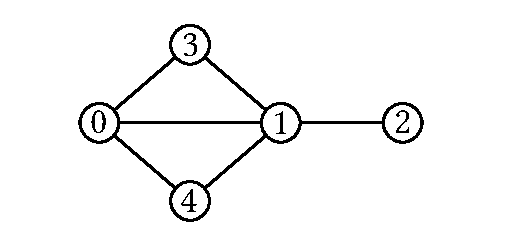
\includegraphics[width=0.7\textwidth]{./architectures/theory/graphs/graph.pdf}}
    \caption{Graphic representation of a graph with five nodes and six edges.}
    \label{fig:five-node-graph-example}
\end{figure}

\begin{equation}
    \label{eq:five-node-graph-adjmatrix}
    A = \left(\begin{matrix}
        0 & 1 & 0 & 1 & 1 \\
        1 & 0 & 1 & 1 & 1 \\
        0 & 1 & 0 & 0 & 0 \\
        1 & 1 & 0 & 0 & 0 \\
        1 & 1 & 0 & 0 & 0 \\
    \end{matrix}\right)
\end{equation}

In the adjacency matrix, the element $A_{ij}$ is set to $1$, if the graph has an edge between the nodes with index $i$ and $j$. 
All $A_{ii}$ here are set to $0$, because generally nodes do not need to be \glqq connected\grqq{} to themselves.

As the graphs inside the neural networks however describe the flow of information, it is quite sensible to assume that the information from one node in one step should somehow be taken into account when generating the information for the next step.
Because of that, it is useful to define multiple adjacency matrices, each with a different purpose.

In \autoref{eq:adjacency-matrix-split}, the adjacency matrices for \emph{self-reference}, \emph{nearest-neighbor-reference} and \emph{next-nearest-neighbor-reference} are shown, referring to the graph in \autoref{fig:five-node-graph-example}. By chance almost every node happens to be a nnn for every node. Only $1$ and $2$ do not have this property. 
For graphs of bigger size, the matrices are generally quite likely to be highly sparse.

\begin{equation}
    \label{eq:adjacency-matrix-split}
    A_\mathrm{self} = \left(\begin{matrix}
        1 & 0 & 0 & 0 & 0 \\
        0 & 1 & 0 & 0 & 0 \\
        0 & 0 & 1 & 0 & 0 \\
        0 & 0 & 0 & 1 & 0 \\
        0 & 0 & 0 & 0 & 1 \\
    \end{matrix}\right)\qquad
    A_\mathrm{nn} = \left(\begin{matrix}
        0 & 1 & 0 & 1 & 1 \\
        1 & 0 & 1 & 1 & 1 \\
        0 & 1 & 0 & 0 & 0 \\
        1 & 1 & 0 & 0 & 0 \\
        1 & 1 & 0 & 0 & 0 \\
    \end{matrix}\right)\qquad
    A_\mathrm{nnn} = \left(\begin{matrix}
        0 & 1 & 1 & 1 & 1 \\
        1 & 0 & 0 & 1 & 1 \\
        1 & 0 & 0 & 1 & 1 \\
        1 & 1 & 1 & 0 & 1 \\
        1 & 1 & 1 & 1 & 0 \\
    \end{matrix}\right)
\end{equation}

To simulate the information exchange at different rates, the matrices can be weighted with different factors. 
\autoref{eq:weighted-adjacency-matrix} shows an adjacency matrix that allows for information to be taken in from the nn, while valuing the current value of the node proportionally higher. 

\begin{equation}
    \label{eq:weighted-adjacency-matrix}
    A_\mathrm{weighted} = 0.9 \cdot A_\mathrm{self} + 0.2 \cdot A_\mathrm{nn} + 0 \cdot A_\mathrm{nnn} = 
    \left(\begin{matrix}
        0.9 & 0.2 & 0 & 0.2 & 0.2 \\
        0.2 & 0.9 & 0.2 & 0.2 & 0.2 \\
        0 & 0.2 & 0.9 & 0 & 0 \\
        0.2 & 0.2 & 0 & 0.9 & 0 \\
        0.2 & 0.2 & 0 & 0 & 0.9 \\
    \end{matrix}\right)\qquad
\end{equation}

Note that as the number of neighbors is not fixed and the accumulated values get added together, the result generally will vary in magnitude depending on the amount of connected nodes in the relations.

The \emph{averaging adjacency matrix} $\tilde{A}$ gets rid of this behavior.
To generate $\tilde{A}$, the matrices $D$ and subsequently $D^{-\frac{1}{2}}$ (\autoref{eq:edge-counting-matrix}) are needed. 
$D$ is the matrix, that counts to number of edges on the corresponding nodes (still for the graph in \autoref{fig:five-node-graph-example}).
Raising a square matrix to a negative fractional power can not only be defined, but even efficiently computed for purely diagonal matrices. 
The calculation is performed element-wise.
Because the matrix has no entries aside from the main diagonal, the expected properties for this inverse are satisfied for the normal matrix multiplication.

\begin{equation}
    \label{eq:edge-counting-matrix}
    D = \left(\begin{matrix}
        4 & 0 & 0 & 0 & 0 \\
        0 & 5 & 0 & 0 & 0 \\
        0 & 0 & 2 & 0 & 0 \\
        0 & 0 & 0 & 3 & 0 \\
        0 & 0 & 0 & 0 & 3 \\
    \end{matrix}\right)\qquad
    D^{-\frac{1}{2}} = \left(\begin{matrix}
        \frac{1}{\sqrt{4}} & 0 & 0 & 0 & 0 \\
        0 & \frac{1}{\sqrt{5}} & 0 & 0 & 0 \\
        0 & 0 & \frac{1}{\sqrt{2}} & 0 & 0 \\
        0 & 0 & 0 & \frac{1}{\sqrt{3}} & 0 \\
        0 & 0 & 0 & 0 & \frac{1}{\sqrt{3}} \\
    \end{matrix}\right)
\end{equation}

When studying \autoref{fig:five-node-graph-example}, one might notice the edge count is equivalent to the number of edges +1 in \autoref{eq:edge-counting-matrix}.
This can be explained by the fact that the self-connection this time is counted ($A = 1 \cdot A_\mathrm{self} +1 \cdot  A_\mathrm{nn}+0 \cdot  A_\mathrm{nnn}$).
By adapting the relations represented by the adjacency matrices or the weighting factors of \autoref{eq:weighted-adjacency-matrix}, the matrix can be tuned to suit a wide range of intended calculations. 
It is however important, to make sure that every node has at least one neighbor counted in $D$, or a division by zero will occur during the calculation of $D^{-\frac{1}{2}}$, crashing the neural network.

$\tilde{A}$ can then be calculated according to \autoref{eq:a-tilde}. 

\begin{equation}
    \label{eq:a-tilde}
    \tilde{A} = D^{-\frac{1}{2}} \cdot A \cdot  D^{-\frac{1}{2}} \stackrel{(Example)}{=} \,\,\left(\begin{matrix}
        \frac{1}{4} & \frac{1}{\sqrt{5}\cdot\sqrt{4}} & 0 & \frac{1}{\sqrt{3}\cdot\sqrt{4}} & \frac{1}{\sqrt{3}\cdot\sqrt{4}} \\
        \frac{1}{\sqrt{4}\cdot\sqrt{5}} & \frac{1}{5} & \frac{1}{\sqrt{2}\cdot\sqrt{5}} & \frac{1}{\sqrt{3}\cdot\sqrt{5}} & \frac{1}{\sqrt{3}\cdot\sqrt{5}} \\
        0 & \frac{1}{\sqrt{5}\cdot\sqrt{2}} & \frac{1}{2} & 0 & 0 \\
        \frac{1}{\sqrt{4}\cdot\sqrt{3}} & \frac{1}{\sqrt{5}\cdot\sqrt{3}} & 0 & \frac{1}{3} & 0 \\
        \frac{1}{\sqrt{4}\cdot\sqrt{3}} & \frac{1}{\sqrt{5}\cdot\sqrt{3}} & 0 & 0 & \frac{1}{3} \\
    \end{matrix}\right)
\end{equation}

It was previously stated, that this thesis is supposed to experiment on an unification of the \emph{metaformer} \cite{metaformerPaper} and \emph{graph networks}.
The question therefore is, how the concept of the adjacency matrix is supposed to be applied to the metaformer framework.\\

\paragraph{Graph convolutions} can be implemented with the knowledge of how to generate the adjacency matrix.
Imagine an intermediate state of a \emph{conformer} to be in the form $b\times h\times w \times e$, where $b$ is the batch dimension, $h$ is the height of the image in patches, $w$ the corresponding width and $e$ the embed dimension (corresponding to the channel dimension $c$ of a depthwise convolution).
For a \emph{depthwise convolution} in a conformer, $e$ 2D-convolutions (one for each channel) would be applied along the axis $h$ and $w$. 
It is now a simple step to transition to the graph version of that problem.
For the \emph{graph conformer}, the intermediate state has the shape $b\times (h\cdot w) \times e = b\times n \times e$, where $h\cdot w = n$ is the number of nodes. 
It is also the side length of the adjacency matrix $A$ for the corresponding graph. 
Comparing \autoref{eq:how-to-compute-symm-conv} and \autoref{eq:weighted-adjacency-matrix} it should become clear that for an image, the depthwise symmetric convolution can be represented by the information in an adjacency matrix that is assembled from $A_\mathrm{self}$, $A_\mathrm{nn}$ and $A_\mathrm{nnn}$ if the correct weights $w_i$ are chosen. This is visualized in \autoref{fig:transition-convolution-graph}.

\begin{figure}[htbp]
    \centering
    \makebox[\textwidth][c]{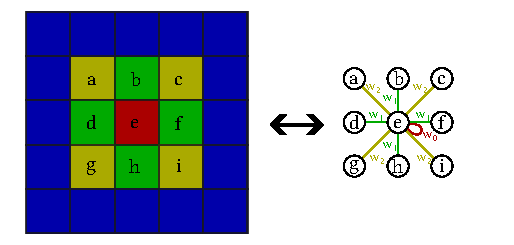
\includegraphics[width=0.8\textwidth]{./architectures/theory/graphs/convolution-comparison.pdf}}
    \caption{Schematic representation that shows the parallels between a depthwise convolution (only one channel shown) of a $3\times 3$ Kernel over a patched image and the corresponding graph. Not involved nodes as well as edges are omitted from the graph on the right side. Both representations show only a subset of the whole situation, as only the calculation for the convolution of node $e$ is shown. The calculations for the other nodes are performed analogously, but shifted to another center patch. When comparing to \autoref{eq:weighted-adjacency-matrix}, $w_0=0.9$, $w_1=0.2$ and $w_2=0$, but with the proper adjacency matrices.
    The color scheme for neighbor visualization is the same as in the \nameref{appendix:lattice-visualisation}.}
    \label{fig:transition-convolution-graph}
\end{figure}

The intermediate state for one element in the batch has the shape $n \times e$. 
That means the shape is $n \times 1$ if only one channel is calculated.
Conveniently, the matrix multiplication of $(n\times n) \cdot (n\times 1)$ is not only possible, but it also gives the correct output dimension of $(n\times 1)$ and the exact same calculation is performed as in a regular symmetric convolution.

When trying to perform the depthwise convolution for an input dimension of $e$, $3 \cdot e$ weights are used ($w_0$,$w_1$ and $w_2$ for each channel, while there are $e$ channels).
This can be evaluated by assembling the adjacency matrix that represents the symmetric convolution from each of the $e$ channels from the matrices $A_\mathrm{self}$, $A_\mathrm{nn}$ and $A_\mathrm{nnn}$ in conjunction with the corresponding three weights.
It is however more efficient to perform the matrix multiplication for each of the three different adjacency matrices only once and spread the result $e$ times. 
Then scaling the results with the weights and finally adding.
The results are the same, because of the distributivity property of matrix multiplication.
This is shown in \autoref{eq:matrix-calculation-distributivity}, assuming the intermediate state at step $t$ is named $v^{(t)}$.

\begin{equation}
    \label{eq:matrix-calculation-distributivity}
    \begin{split}
        v^{(t+1)}_{b=i, e=j} &= \left[\left(w_{0, j} \cdot A_\mathrm{self} + w_{1, j} \cdot A_\mathrm{nn} + w_{2, j} \cdot A_\mathrm{nnn}\right) \cdot v^{(t)}_{b=i}\right]_{e=j}\\
        &= \left[w_{0, j} \cdot \left(A_\mathrm{self}\cdot v^{(t)}_{b=i}\right) + w_{1, j} \cdot \left(A_\mathrm{nn}\cdot v^{(t)}_{b=i}\right) + w_{2, j} \cdot \left(A_\mathrm{nnn}\cdot v^{(t)}_{b=i}\right)\right]_{e=j}
    \end{split}
\end{equation}

The jax style implementation for this calculation can be seen in the appendix at \ref{appendix:graph-conformer}.

\paragraph{Graph pooling} is basically implemented analogously to the graph convolution.
However it utilizes the averaging matrix $\tilde{A}$ (\autoref{eq:a-tilde}) instead, in order to simulate an \emph{average pooling} operation.
As pooling does not require different or trainable weights along the axis $e$, the matrix can be pre-computed and cached.
The jax style implementation is printed in the appendix at \ref{appendix:graph-poolformer}.


\paragraph{Graph attention} is the metaformer token mixer requiring the least modifications.
In \cite{swinTransformerPaper} the transformer attention is limited to non-uniform, local blocks, by only calculating parts of the outer multiplication in the scaled dot product attention algorithm (\autoref{eq:attention-step-2}).

Here a more complex relationship of the patches is pictured. 
The dimensionality of the outer product matrix $M$ (from \autoref{eq:attention-step-2}) and the adjacency matrix for the encoded graph match.
This is no coincidence, as the entry $M_{ij}$ corresponds to the attention from patch $i$ onto patch $j$, while $A_{ij}$ is a measure for how \glqq connected\grqq{} the patches are according to the graph structure.
\emph{Graph attention} is therefore calculated as the element-wise multiplication of $M$ and $A$.
Because of the element-wise multiplication, it is not sensible to use $\tilde{A}$, which is motivated by matrix multiplication.
Before passing the masked values through the softmax function, all zero values need to get set to $-\infty$.
By doing that, it is ensured their contribution to the softmax evaluates to 0 and the corresponding connection is therefore masked out completely.
The element wise multiplication and replacement with $-\infty$ happens on line 162 of the attention algorithm implementation in jax style (appendix, \ref{appendix:attention}).

\paragraph{Graph patching} can be achieved in multiple different ways.
In order to get the input configuration into a state that is processable by transformers, the input shape needs to have the dimension $n \times e$, with the number of lattice sites $n$ and the embed dimension $e$.
To achieve this, a state encoding of shape $n \times x$ is generated from the randomly sampled spin state $s_\mathrm{input} \in \{0,1\}^n$.
$x$ depends on the chosen \emph{embed\_mode} strategy (\emph{duplicate\_spread}, \emph{duplicate\_nn} or \emph{duplicate\_nnn}), as well as the lattice shape. 
An example for the different strategies is displayed in \autoref{fig:graph-patching}.

\begin{figure}[htbp]
    \centering
    \makebox[\textwidth][c]{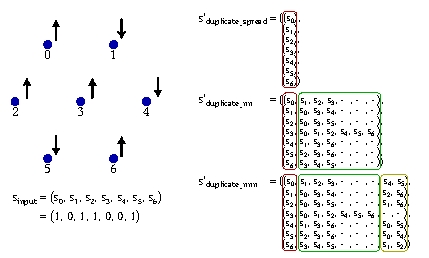
\includegraphics[width=\textwidth]{./architectures/theory/graphs/patching.pdf}}
    \caption{Assembling of the transformed inputs $s'$ of shape $n\times x$. $x$ depends on the embed\_mode strategy.
                The intermediate step's shape further depends on the shape of the chosen lattice. 
                In the example, a trigonal\_hexagonal lattice of size 1 is chosen.
                The color scheme for neighbor visualization is the same as in the \nameref{appendix:lattice-visualisation}.}
    \label{fig:graph-patching}
\end{figure}

To convert the intermediate state $s'$ into the final form, the values are newly assigned
($1 \rightarrow 1,\quad 0\rightarrow -1,\quad (-) \rightarrow 0$). 
To be easier for the network to differentiate, (0,1) is mapped to (-1,1) and previously unassigned vales are set to 0.

To reshape the element of size $n \times x$ to the input $n\times e$, a fcl is used.
This strategy is analogous to the patching algorithm of most vision transformers.

The mapping pictured in \autoref{fig:graph-patching} can be performed quite efficiently by using a helper matrix and applying one \emph{einsum} operation.  
The details can be referenced in the code \cite{selfPhysics}.

